\documentclass[paper=a4,fontsize=11pt,parskip=half]{scrartcl}

%% packages
\usepackage[ngerman]{babel}
\usepackage{fontspec}
\usepackage{lmodern}
\usepackage{color}
\usepackage{graphicx}
\usepackage[autostyle=true,german=quotes]{csquotes}
\usepackage[hidelinks=true,colorlinks=false]{hyperref}
\usepackage{listings}
\usepackage[export]{adjustbox} % For frames with includegraphics
\usepackage{pgfgantt}
\usepackage{framed}
\usepackage[a4paper, top=1in]{geometry}
\usepackage{todonotes}

\newcommand*\circled[1]{\tikz[baseline=(char.base)]{
    \node[shape=circle,draw,inner sep=2pt] (char) {#1};}}

\definecolor{darkgray}{rgb}{.2,.2,.2}

\lstset{basicstyle=\footnotesize\ttfamily,breaklines=true}

\lstdefinelanguage{Grammar}{
  keywords={grammar, typedef, node, prop, terminal, children},
  keywordstyle=\color{blue},
  ndkeywords={string, boolean, between, allowed, sequence},
  ndkeywordstyle=\color{black},
  identifierstyle=\color{black},
  sensitive=false,
  commentstyle=\color{purple}\ttfamily,
  stringstyle=\color{red}\ttfamily,
  morestring=[b]',
  morestring=[b]"
}

\title{Generierung von syntaxfreien Entwicklungsumgebungen für beliebige Programmiersprachen}
\author{Marcus Riemer}

\makeatletter
\hypersetup{
  pdftitle={\@title},
  pdfauthor={\@author}
}
\makeatother

\usepackage[backend=biber,defernumbers=true,sorting=none]{biblatex}
\addbibresource[datatype=bibtex]{diss.bib}

\AtEveryBibitem{
  \clearfield{urlyear}
  \clearfield{urlmonth}
}

\setcounter{biburllcpenalty}{7000}
\setcounter{biburlucpenalty}{8000}

\begin{document}
\pagenumbering{gobble}
\pagestyle{empty}

\maketitle
\tableofcontents

\clearpage
\pagenumbering{roman}
\newgeometry{bottom=1in, top=1in}
\section{Einseitige Kurzfassung}

Bildungs-Politiker und -Forscher sehen grundlegende Programmierkenntnissen als Teil der Allgemeinbildung und wollen entsprechenden Unterricht an Schulen zum verpflichtenden Inhalt machen \cite{noauthor_designierte_2018}. Die Lehrkräfte welche diese Anforderungen umzusetzen haben, stehen aber vor einem Problem: Konventionelle Programmierwerkzeuge sind speziell auf die Bedürfnisse von professionellen Anwendern zugeschnitten. Aufgrund der damit verbundenen Komplexität eignen sich diese Programmierwerkzeuge aus didaktischer Sicht nur eingeschränkt für die Einführung in die Programmierung. Außerdem haben Studien gezeigt, dass die strengen syntaktischen Anforderungen von gängigen Programmiersprachen eine hohe Einstiegshürde darstellen können \cite{resnick_scratch:_2009}. Trotzdem kommen die professionellen Werkzeuge, in der Regel aus Mangel an Alternativen, häufig im Unterricht zum Einsatz. Darüber hinaus sind viele der ersten Aufgaben weit von der Lebenswirklichkeit der Lernenden entfernt, was sich negativ auf deren Motivation auswirken kann \cite{resnick_scratch:_2009}.

Im Rahmen dieser Promotion soll erforscht und demonstriert werden, wie sich aus formalen Beschreibungen von Programmiersprachen benutzerfreundliche syntaxfreie Entwicklungsumgebungen erzeugen lassen. Letztendlich soll Lehrkräften ein Werkzeug an die Hand gegeben werden, welches die erwähnte Einstiegshürde in die Programmierung mit konventionellen Programmiersprachen wie \texttt{SQL}, \texttt{HTML}, \texttt{CSS} oder \texttt{JavaScript} senkt. Und Lernende sollen unter Anleitung schnell motivierende Projekte wie interaktive Webseiten umsetzen und letztlich den Schritt zu konventionellen Werkzeugen machen können.

Die erzeugten Editoren sollen im Regelfall das Erscheinungsbild existierender Sprachen imitieren. Obwohl die Darstellung eines im Editor bearbeiteten Programms also große Nähe zur textuellen Darstellung haben kann, erfolgt die Programmierung per Maus durch das Verschieben der dargestellten Blöcke. Dieses Bedienkonzept orientiert sich an den Erfahrungen, welche die Forscher hinter Projekten wie \textit{Scratch}~\cite{maloney_scratch:_2004} oder Googles \textit{Blockly}~\cite{fraser_ten_2015} gemacht haben. Abbildung~\ref{fig:example-sql-ide} zeigt ein prototypisches Beispiel für einen generierten \texttt{SQL}-Editor\footnote{Dieser und weitere Prototypen lassen sich unter \url{https://blattwerkzeug.de/villigst} ausprobieren.}. Die reale Programmiersprache lässt sich erkennen, obwohl deren Syntaxanteile vom Anwender nicht geschrieben werden musste. Anders als in \textit{Scratch} oder \textit{Blockly} könnten die Programme 1:1 abgetippt werden und würden funktionieren.

Der gewählte Ansatz, also die Generierung von Editoren, ermöglicht es Lehrkräften außerdem die im Rahmen der Promotion erarbeiteten (und möglicherweise für die Lernziele zu umfangreichen) Editoren didaktisch einzuschränken. In Anlehnung an die bei \cite{klaeren_macht_2007} beschriebenen \enquote{Sprachebenen} lässt sich also der Funktionsumfang der von Lehrkräften generierten Editoren an den Lernfortschritt der Klassengemeinschaft anpassen.

\begin{figure}[h]
  \centering\includegraphics[width=\linewidth]{screenshot-drag-drop-ide.png}
  \caption{Generierter Editor für die Programmiersprache \texttt{SQL}, die gezeigte Abfrage sucht in Titeln aus der Buchserie \enquote{Die drei Fragezeichen}.}
  \label{fig:example-sql-ide}
\end{figure}

\clearpage

\pagenumbering{arabic}
\restoregeometry
\pagestyle{plain}

\section{Detaillierte Konzeption}

Die im Rahmen der Arbeit erstellten Ergebnisse sind sowohl theoretischer als auch praktischer Natur. Viele der aufzustellenden Hypothesen betreffen subjektive Qualitätsmerkmale und lassen sich daher nicht eindeutig quantifizieren oder ohne Versuche mit Probanden sinnvoll bewerten. Daher soll die praktische Implementierung eben jene Annahmen durch Demonstrationen oder Tests mit Probanden untermauern oder widerlegen. Das Projekt befindet sich damit in einem etwas ungewöhnlichen Spannungsfeld zwischen der klassischen Informatik-Kerndisziplin Übersetzerkonstruktion (Compilerbau) und der Informatik-Didaktik. Darüber hinaus spielen auch Aspekte der Mensch-Computer-Interaktion eine Rolle, schließlich geht es neben der Übersetzung der Programme vor allem um die Konstruktion benutzerfreundlicher Schnittstellen.

\begin{framed}
  \textbf{Hinweis}: Der Prototyp kann unter \href{https://blattwerkzeug.de}{\texttt{blattwerkzeug.de}} ausprobiert werden.
\end{framed}

\subsection{Syntaxfreie Programmiersprachen}

Bei syntaxfreien Programmiersprachen muss der Programmierer sich nicht mit den syntaktischen Details der verwendeten Programmiersprache beschäftigen. Bei einer solchen Programmiersprache ist es irrelevant, ob zum Beispiel Anweisungen durch Semikola getrennt werden, Blöcke mit geschweiften Klammer, \texttt{begin} und \texttt{end} oder durch Leerraum definiert werden oder welche Klammern an welcher Stelle notwendig sind.

In der Praxis handelt es sich bei solchen syntaxfreien Sprachen de facto immer um visuelle Programmiersprachen. Auch die schon erwähnten Umgebungen \textit{Scratch} und \textit{Blockly} fallen in diese Kategorie. In diesen Umgebungen arbeitet der Programmierer mit der Maus um die verschiedenen zur Verfügung stehenden Blöcke an syntaktisch zulässigen Orten zu platzieren. Diese Art der Programmierung ist für erfahrene Programmierer oder umfangreiche Softwareprojekte erfahrungsgemäß hinderlich \cite[S. 262f]{schiffer_visuelle_2001}, eignet sich aber zur Einführung in die Programmierung \cite{resnick_scratch:_2009}.

\subsection{Vorherige Arbeit: Master-Thesis}

Die Masterthesis \enquote{BlattWerkzeug} \cite{riemer_blattwerkzeug_2016}  wurde im Oktober 2016 vom Bewerber Marcus Riemer fertiggestellt und beschreibt zwei konkrete syntaxfreie Editoren für \texttt{SQL} und \texttt{HTML}. Diese Master-Thesis legte in ideeller Weise den Grundstein für das Promotionsvorhaben und demonstrierte, dass sich eine Entwicklungsumgebung für Schüler prinzipiell auch von nur einem Entwickler umsetzen ließe. Aus technischer Sicht handelte es sich aber um eine sehr spezifische und eher unflexible Lösung. Im Februar 2018 wurde daher der gesamte Code für diese konkreten Editoren neu erstellt und durch einen ersten Prototypen des im folgenden beschriebenen neuen, generativen Ansatzes ersetzt \cite{riemer_commit_2018}.

Dieses Promotionsvorhaben versteht sich damit als eine Iteration des ursprünglichen Ansatzes: Anstatt jede weitere zu unterstützende Programmiersprache mühsam von Grund auf neu zu entwickeln, soll die Integration weiterer Sprachen mit etablierten Techniken und Vorgehensweisen aus der normalen Übersetzerkonstruktion vorgenommen werden können. Der Ansatz der Thesis erfordert für jede Veränderung der bereitgestellten Editoren einen fachlichen Experten mit Erfahrung in dieser sehr speziellen Software (konkret: Marcus Riemer). Der neue Ansatz hingegen ermöglicht es erfahrenen Anwendern (zum Beispiel Lehrkräften) Variationen von bestehenden Editoren zu erzeugen. Dieses Vorgehen orientiert sich an bestehenden Modellierungsumgebungen wie zum Beispiel Eclipse \textit{xText} \cite{efftinge_oaw_2006}, diese erzeugen allerdings klassische textuelle Editoren statt syntaxfreier Editoren.

\subsection{Eingrenzung und Wahl des Forschungsvorhabens}

Es handelt sich bei diesem Promotionsvorhaben -- trotz der möglichen praktischen Anwendungen in der Informatik-Lehre -- ausdrücklich nicht um eine didaktische Arbeit. Es findet folglich keine didaktisch fundierte Konzeption von möglichen Lehrinhalten oder Unterrichtsstunden statt.

Diese Einschränkung ist zum Einen durch den fachlichen Hintergrund der Beteiligten bedingt: PD Dr. Frank Huch als Erstgutachter und Betreuer ist Informatiker und arbeitet an der CAU Kiel im Fachbereich \textit{Programmiersprachen und Übersetzerkonstruktion}. Der Promotionsstudent Marcus Riemer ist ebenfalls Informatiker und arbeitet als wissenschaftlicher Mitarbeiter an der Fachhochschule Wedel. Beiden gemein ist das Anliegen, eine möglichst frühe und effektive Vermittlung von Informatik-Kenntnissen an Schulen möglich zu machen. Auch wenn es ihrer Einschätzung nach möglich wäre, aufbauend auf der Masterthesis eine vornehmlich didaktische Arbeit zu schreiben, würde dies eine umfangreiche Einarbeitung in die entsprechenden didaktischen Hintergründe und Methoden voraussetzen. Diese Einarbeitungzeit entfällt durch die Fokussierung auf Fragestellungen und Themen aus der Informatik -- dem eigenen Fachgebiet.

Zum Anderen halten Dr. Huch und Herr Riemer den gewählten Schwerpunkt, also die automatische Erzeugung von benutzerfreundlichen Editoren, für wissenschaftlich und praktisch grundlegender. Unserem Wissensstand nach existiert noch keine Software, welche die Vorgehensweise aus der Übersetzerkonstruktion zur automatisierten Generierung von syntaxfreien Editoren verwendet. Und auch die im Rahmen der Promotion erstellte Software soll selbstverständlich von Experten und Forschern mit didaktischem Hintergrund untersucht und begleitet werden. Es ist vorgesehen, die zu erstellende Software von Lehramtsstudierenden der CAU Kiel, von den Kollegen der Kieler Arbeitsgruppe Didaktik der Informatik, im Rahmen von Lehrerfortbildungen oder auch direkt an Schulen im Informatikunterricht auf ihre Eignung für den Unterrichtsgebrauch zu prüfen.

\subsection{Technische Konzeption}

Um einen möglichst einfachen Zugang zur Software für Lernende zu gewährleisten, wird der praktische Teil des Projekts als Webanwendung entwickelt. Für die ersten Schritte der Softwareentwicklung reicht auf Seiten der Lernenden dann ein aktueller Browser. Mit diesem Ansatz ist das Vorhaben in guter Gesellschaft: Das Vorbild \textit{Scratch} ist ebenfalls über den Browser erreichbar, genau so wie auch mit \textit{Blockly} erzeugte Umgebungen \cite[vgl. S. 28]{riemer_blattwerkzeug_2016}.

Abbildung~\ref{fig:core-relations} veranschaulicht zentrale Begriffe des Vorhabens und deren Zusammenhänge. Auf der obersten Ebene sind beim Editieren eines Programms mit einem syntaxfreien Block-Editor (siehe Abbildung~\ref{fig:example-sql-ide} aus der Einleitung für ein Beispiel) fünf grundlegende Datenstrukturen involviert:

\begin{figure}
  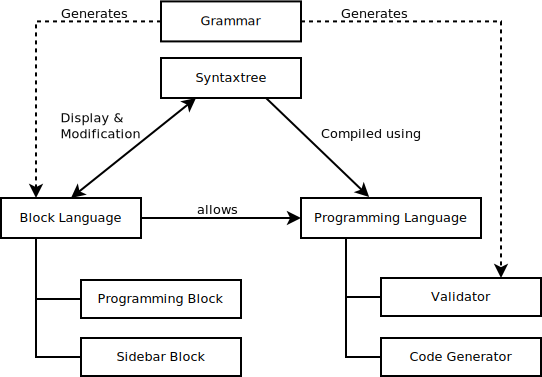
\includegraphics[width=\linewidth]{core-concepts.pdf}
  \caption{Zusammenhänge der zentralen Begrifflichkeiten}
  \label{fig:core-relations}
\end{figure}

\begin{itemize}
\item Die \textbf{Grammatik} (Grammar) definiert die grundsätzlich zulässigen Strukturen eines abstrakten Syntaxbaums. Aus dieser Beschreibung lassen sich unmittelbar Validatoren zur Überprüfung von Syntaxbäumen erzeugen. Nimmt man zu dieser Beschreibung noch spezielle \textbf{Generator-Anweisungen} (Generator Instructions) dazu, können aus einer Grammatik auch Blocksprachen erzeugt werden.
\item Der \textbf{abstrakte Syntaxbaum} (Syntaxtree, AST) repräsentiert die Struktur eines Quelltextes der mit einem Blockeditor bearbeitet wird. In einer konventionellen Entwicklungsumgebung würde man an dieser Stelle von einer \textit{Datei} sprechen.
\item Die \textbf{Blocksprache} (Block Language) weiß wie die zu bearbeitende \textit{Datei} (also ein Syntaxbaum) darzustellen ist. Hier wird definiert wie die einzelnen Teile des Syntaxbaumes visualisiert und editiert werden sollen (also den konkreten Editor) und welche Blöcke dem Benutzer angeboten werden. Außerdem können zu einer Blocksprache auch sprachspezifische Komponenten gehören, zum Beispiel die Anzeige von Abfrageergebnissen bei \texttt{SQL} oder ein Terminal zur Ein- und Ausgabe.
\item Die tatsächliche Kompilierung, Validierung und Ausführung erfolgt anhand einer \textbf{Programmiersprache} (Programming Language). Im Regelfall wird Quelltext für real existierende Zielsprachen wie \texttt{SQL} oder \texttt{JavaScript} erzeugt, welcher dann in einer speziellen Laufzeitumgebung auf dem Server ausgeführt wird.
\end{itemize}

Für normale Nutzer, also vornehmlich Lernende, sind diese Unterscheidungen nicht von Bedeutung. Aus ihrer Sicht interagieren sie im Browser mit einer Art Dateibaum und bekommen automatisch, passend zum Typ der \enquote{Datei}, entsprechende Entwicklungsumgebungen präsentiert.

Darüber hinaus kann durch die konsequente Verwendung eines abstrakten Syntaxbaumes der für andere Compiler typische Parsing-Vorgang entfallen. Anwender sollen Programme mit den generierten syntaxfreien Editoren erstellen und editieren, nicht in einem Texteditor. Die Aufgabe des generierten Editors ist somit die Darstellung und Bearbeitung von Syntaxbäumen.

\subsubsection{Der abstrakte Syntaxbaum}

Der Syntaxbaum als solcher ist nichts weiter als eine Datenstruktur, auf welcher Operationen zur Veränderung (einfügen, löschen, tauschen, ...) definiert sind. Der Baum verfügt explizit über keinerlei Funktionalität zur eigenen Validierung oder zur Erzeugung von Programmcode. Er fungiert stattdessen als Eingabe für andere Module, welche diese Funktionalität bereitstellen.

Jeder Knoten eines Baums entspricht mindestens einem Typen, welcher sich aus den Zeichenketten \texttt{language} (im Sinne einer Programmiersprache) und \texttt{name} zusammensetzt. Anhand dieses Typs entscheiden alle anderen Module wie genau mit dem Knoten zu verfahren ist. Durch die Aufteilung des Typen in einen lokalen Namen und einen Namensraum lassen sich potenzielle Namenskollisionen vermeiden. Der einfachste denkbare Baum besteht aus einem einzigen Knoten mit ausschließlich einer Typangabe. Abbildung~\ref{fig:ast-example-null} zeigt wie sich ein Ausdruck, welcher aus nichts weiter als dem symbolischen Wert \texttt{null} besteht, für eine nicht näher benannte Sprache als Syntaxbaum ausdrücken ließe.

Die Speicherung von atomaren Daten erfolgt im Syntaxbaum durch die Verwendung so genannter \textit{Eigenschaften} (engl. \textit{Properties}). Dabei handelt es sich um Zeichenketten, Zahlen oder Wahrheitswerte welche über einen Schlüssel zugreifbar sind. Die Abbildungen~\ref{fig:ast-example-variable}, \ref{fig:ast-example-binary} und \ref{fig:ast-example-if} zeigen wie solche Eigenschaften in Knoten zum Einsatz kommen können.

Kinder von Knoten werden in benannten \textit{Kindgruppen} organisiert. Dabei handelt es sich um eine Verallgemeinerung der von \texttt{XML} bekannten Aufteilung in Attribut-Kinder und Element-Kinder. Mit diesen Syntaxbäumen lassen sich die Kinder folglich beliebig in Unterbäumen organisieren. Die Abbildungen~\ref{fig:ast-example-binary} und \ref{fig:ast-example-if} illustrieren, wie Unterbäume genutzt werden können um binäre Ausdrücke oder eine \texttt{if}-Anweisung darzustellen.

Die Einführung dieser eher ungewöhnlichen Konstrukte (\textit{Eigenschaften} und \textit{Kindgruppe}) dient der Vermeidung von künstlichen Knoten. Theoretisch wäre es problemlos möglich die Organisation von Unterbäumen durch z.B. speziell benannte künstliche Knoten vorzunehmen. Und auch atomare Werte könnten in Blattknoten gespeichert werden. Die Aufgabe dieses speziellen Syntaxbaums ist jedoch nicht nur die Persistierung: Der Baum ist auch die Datenstruktur, welche die generierten Editoren anzeigen und auf denen die Anwender ihre Veränderungen vornehmen. Dabei hat es sich als hilfreich erwiesen auf Knoten zu verzichten, für die sich keine eigene Darstellung im Editor finden lässt.

\begin{figure}[p]
  \centering\includegraphics{ast-example-null.pdf}
  \caption{Syntaxbaum für \texttt{null}-Werte in einer nicht näher beschriebenen Sprache \texttt{lang}. Dieser Knoten enthält außer seinem Typnamen keine Daten.}
  \label{fig:ast-example-null}
\end{figure}

\begin{figure}[p]
  \centering\includegraphics{ast-example-expr-variable.pdf}
  \caption{Baum für den Einsatz einer Variablen \texttt{numRattles}, z.B. als Teil eines Ausdrucks. Der Name der referenzierten Variable ergibt sich aus dem Wert der Eigenschaft \texttt{name}.}
  \label{fig:ast-example-variable}
\end{figure}

\begin{figure}[p]
  \centering\includegraphics{ast-example-expr-binary.pdf}
  \caption{Baum für den Vergleich einer Variablen \texttt{numRattles} mit \texttt{null}. Die Art des Vergleichs ergibt sich aus der Eigenschaft \texttt{op} des Wurzelknotens. Die Reihenfolge der Operanden folgt aus den Namen der Kindgruppen (\texttt{rhs} = right hand side, \texttt{lhs} = left hand side).}
  \label{fig:ast-example-binary}
\end{figure}

\begin{figure}[p]
  \centering\includegraphics[width=\textwidth]{ast-example-if.pdf}
  \caption{Baum für eine \texttt{if}-Anweisung mit zwei alternativ möglichen Funktionsaufrufen. Die Kindgruppe \texttt{pred} (Prädikat) steht dabei für den Wahrheitsausdruck, \texttt{positive} für den positiven Zweig und \texttt{negative} für den negativen Zweig.}
  \label{fig:ast-example-if}
\end{figure}

\subsubsection{Die Grammatiken}
\label{sec:grammars}

Die für dieses Promotionsvorhaben notwendigen Grammatiken unterscheiden sich in zwei wesentlichen Aspekten von gängigen Grammatiken, wie sie in der Übersetzerkonstruktion zum Einsatz kommen \cite[S. 42ff]{aho_compilers:_2007}:

\begin{enumerate}
\item Die zu verarbeitende Eingabe ist keine Zeichenkette, sondern ein bestehender Syntaxbaum. Da alle Operationen grundsätzlich auf Syntaxbäumen stattfinden, orientiert sich die Arbeitsweise der Grammatik an bestehenden Schemasprachen zur Validierung von Bäumen, konkret an RELAX NG \cite{clark_relax_2001}. Aufgabe einer Grammatik im Rahmen dieses Vorhabens ist folglich nicht die Unterstützung des Parsing-Vorgangs, sondern die Validierung bestehender Syntaxbäume.
\item Aus der Grammatik heraus sollen Oberflächen generiert werden, allerdings sind die für die Validierung bereitgestellten Informationen alleine nicht ausreichend, um daraus sinnvolle Oberflächen zu generieren. Welche Annotationen notwendig oder hilfreich sind und wo diese Annotation vermerkt werden sollen, ist Bestandteil der zu untersuchenden Fragestellungen. Für Generatoren von textbasierte Editoren stellt sich diese Frage hingegen nicht: Eingabe und Codevervollständigung können immer nach etablierten Mustern vorgenommen werden.
\end{enumerate}

Das folgende Beispiel leitet eine Grammatik her, welche sich zunächst zur Validierung von \texttt{XML}-artigen Sprachen eignen würde. Wir beginnen dafür in Listing~\ref{lst:xml-grammar-1} mit der Definition einer Grammatik, welche lediglich Bäume mit einem benannten Element als valide auffassen würde.

\begin{lstlisting}[float=h, label={lst:xml-grammar-1},caption={\texttt{XML} Schritt 1 - Elemente mit Namen},captionpos=b,language={Grammar}]
grammar "xml" {
  node "element" {
    prop "name" { string }
  }
}
\end{lstlisting}

Die Definition eines erlaubten Knotens wird mit \texttt{node} eingeleitet, der im Syntaxbaum zu verwendende Typname ergibt sich aus dem Namen der Grammatik (\texttt{xml}) und dem Namen des Knotens (\texttt{element}). In diesem konkreten Fall darf ein valider Knoten lediglich über eine einzige Eigenschaft (\texttt{prop(erty)}) \texttt{name} verfügen, nicht jedoch über Kinder oder Attribute. Die mit \texttt{prop} definierte Eigenschaft wird für den Moment nicht weiter eingeschränkt, sondern darf eine beliebige Zeichenkette sein. Ein im Sinne dieser Grammatik valider Baum hätte also einen einzigen Knoten vom Typ \texttt{xml.element} mit einer Eigenschaft \texttt{name}. Die Definition der Attribut-Knoten kann analog zu dem Elementknoten erfolgen (Listing~\ref{lst:xml-grammar-2}). Da es sich bei Attributen um Name-Wert-Paare handelt, kommen an dieser Stelle zwei Eigenschaften zum Einsatz.

\begin{lstlisting}[float=h, label={lst:xml-grammar-2},caption={\texttt{XML} Schritt 2 - Elemente mit Namen, Attribute mit Schlüssel-Wert-Paaren},captionpos=b,language={Grammar}]
grammar "xml" {
  node "element" {
    prop "name" { string }
  }
  node "attribute" {
    prop "name" { string }
    prop "value" { string }
  }
}
\end{lstlisting}

Schlussendlich müssen dann noch die zulässigen Beziehungen zwischen Elementen und Attributen definiert werden: Ein Element darf sowohl Elemente als auch Attribute als Kinder haben, allerdings in verschiedenen Kindgruppen (Listing~\ref{lst:xml-grammar-3}). Die Anweisung \texttt{children} innerhalb einer \texttt{node}-Definition erwartet zunächst die Angabe eines Namens und dann folgt mit \texttt{::=} getrennt eine an Produktionsregeln angelehnte Aufzählung der zulässigen Typen in dieser Kindgruppe.

Innerhalb dieser \enquote{Produktionsregeln} können die Typen mit den bekannten Quantifizierern \texttt{*} (beliebig häufig), \texttt{+} (mindestens ein Mal) und \texttt{?} (optional) versehen werden. Exakte Häufigkeitsangaben sind ebenfalls möglich, die Syntax lehnt sich dabei an die erweiterte Backus-Naur-Form an.

Im konkreten Beispiel (Listing~\ref{lst:xml-grammar-3}) dürfen also beliebig viele andere Elemente oder Attribte als Kindknoten eines \texttt{xml.element}-Knotens auftreten. Es ist dabei allerdings unzulässig einen \texttt{xml.attribut}-Knoten in der Kindgruppe \texttt{elements} zu verwenden und umgekehrt.

\begin{lstlisting}[float=h, label={lst:xml-grammar-3},caption={\texttt{XML} Schritt 3 - Beziehungen zwischen Elementen und Attributen},captionpos=b,language={Grammar}]
grammar "xml" {
  node "element" {
    prop "name" { string }
    children "elements" ::= element*
    children "attributes" ::= attribute*
  }
  node "attribute" {
    prop "name" { string }
    prop "value" { string }
  }
}
\end{lstlisting}

\subsubsection{Validierung}

Die so definierte Grammatik hat in Bezug auf die sich daraus ableitenden Möglichkeiten zur Validierung noch folgende Schwächen:

\begin{enumerate}
\item Die Namen eines Elementes oder die Attributwerte könnten \texttt{XML}-Steuerzeichen wie \texttt{"}, \texttt{<} oder \texttt{>} enthalten. Der Wertebereich von Attributen lässt sich daher auf Basis von regulären Ausdrücken einschränken.
\item Es wäre möglich in der \texttt{attributes}-Kindgruppe eines \texttt{element} zwei \texttt{attribute}-Knoten mit identischen \texttt{name}-Eigenschaften anzugeben. Das entspräche z.B. dem folgenden (illegalen) \texttt{XML}-Knoten: \texttt{<elem key='1' key='2'/>}. Dieser inhaltliche Fehler lässt sich nicht alleine durch die Grammatik bereinigen.
\end{enumerate}

Probleme semantischer Natur, zum Beispiel die Gültigkeit von Bezeichern oder Typprüfungen in Ausdrücken, lassen sich nicht über die Grammatik abbilden. Fehler dieser Art lassen sich häufig nur in einem spezifischen Kontext überprüfen. Für \texttt{SQL}-Abfragen ist die Korrektheit beispielsweise von der konkreten Datenbank abhängig: Nur wenn die erwähnten Tabellen und Spalten dort existieren, lässt sich die Abfrage verwenden. Daher ist es teilweise nötig, ergänzend zu den aus der Grammatik ableitbaren Regeln, noch eigene Validierungsregeln in Form von eigens erstellten Funktionen anzugeben. Diese Regeln können nicht von Lehrkräften formuliert werden, sondern bedürfen die Fachkenntnis eines Informatikers.

\subsubsection{Die Blocksprachen}

Die aus den Grammatiken erzeugten Blocksprachen folgen im aktuellen Prototypen einem festen Übersetzungsschema, um Grammatiken in einen Satz von Bedienelementen, verfügbaren Blöcken und sprachspezifischen Anzeigeelementen umzuwandeln. Die Details dieser Erzeugung sind ein wesentlicher Aspekt der Promotion. Der aktuell im Prototypen implementierte Stand benötigt noch detaillierte manuelle Angaben um Aspekte wie die Einrückung oder die Orientierung von Blöcken sinnvoll zu wählen.

Listing~\ref{lst:xml-grammar-terminals} demonstriert, wie die Definition der Elemente und Attribute aus dem \texttt{XML}-Beispiel um Terminalsymbole erweitert werden könnte. Mit diesen zusätzlichen Angaben kann dann eine Blocksprache erzeugt werden, welche sich sehr nah an die textuelle Repräsentation von XML hält.

\begin{lstlisting}[float=h, label={lst:xml-grammar-terminals},caption={Terminalsymbole für Attribute und Elemente in \texttt{XML} },captionpos=b,language={Grammar}]
grammar "xml" {
  node "element" {
    terminal "tag-open-begin" "<"
    prop "name" { string }
    children "attributes" ::= attribute*
    terminal "tag-open-end" ">"
    children "elements" ::= element*
    terminal "tag-close" "<ende/>"
  }
  node "attribute" {
    prop "name" { string }
    terminal "equals" "="
    terminal "quot-begin" "\""
    prop "value" { string }
    terminal "quot-end" "\""
  }
}
\end{lstlisting}

Grundsätzlich werden die Angaben in der Grammatik in der dort definierten Reihenfolge in Blockdefinitionen übersetzt, welche dann zur Laufzeit interpretiert und schlussendlich als zusammenhängender Editor dargestellt werden. Allerdings entstehen nur auf Basis der \texttt{prop}- und \texttt{children}-Angaben keine Editoren, welche einigermaßen nah an der textuellen Repräsentation der jeweiligen Sprache wären: Es fehlen die Syntaxbestandteile, welche die Orientierung ermöglichen. Deswegen lassen sich die Grammatiken um die Angabe von Terminalsymbolen erweitern. Aus Sicht der Validierung sind diese Daten schlichtweg unnötig -- der Syntaxbaum enthält keine Syntaxbestandteile -- und diese werden dort daher nicht weiter berücksichtigt. Der Generator kann auf Basis dieser Angaben aber Editoren erzeugen, welche sich näher an der Zielsprache orientieren.

Um den einfacheren \texttt{attribute}-Typen in einen Block zu übersetzen, kommen vor allem zwei Bausteine zum Einsatz: Eigenschaften werden in editierbare Eingabefelder umgewandelt und Terminalsymbole in schlichte Texte. Anhand der vergebenen Namen für die Terminalsymbole lassen sich diese auch in der Gestaltung farblich anpassen. Abbildung~\ref{fig:ast-example-xml-node-two-attributes} zeigt einen konkreten Syntaxbaum, welcher in einem generierten Editor in Abbildung~\ref{fig:example-xml-generated} dargestellt wird. Im gezeigten Zustand hat der Benutzer den Attribut-Schlüssel \texttt{att1} angeklickt und kann nun den \texttt{name}-Eigenschaftswert eines \texttt{xml.attribute}-Knotens bearbeiten. Die Terminalsymbole wurden für die Darstellung exakt aus der Grammatik (Listing~\ref{lst:xml-grammar-terminals}) übernommen.

\begin{figure}[h]
  \centering\includegraphics{ast-example-xml-node-two-attributes.pdf}
  \caption{Syntaxbaum für einen \texttt{XML}-Baum mit einem Element welches zwei Attributge hat: \texttt{<parent att1='Neuer Text' a2='' />}.}
  \label{fig:ast-example-xml-node-two-attributes}
\end{figure}

\begin{figure}[h]
  \centering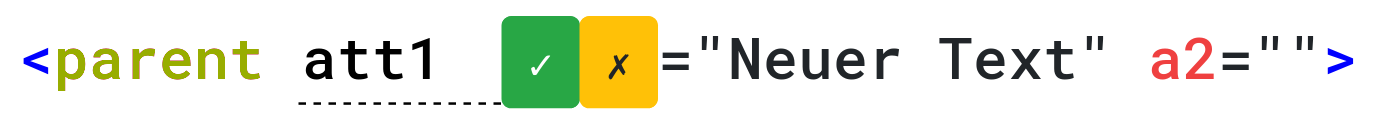
\includegraphics[width=\linewidth]{screenshot-generated-xml.png}
  \caption{Visualisierter Syntaxbaum (Abbildung~\ref{fig:ast-example-xml-node-two-attributes}) auf Basis der gezeigten Grammatik (Listing~\ref{lst:xml-grammar-terminals}) und zusätzlicher Farbangaben aus den Generator-Anweisungen (Abbildung~\ref{fig:block-lang-generation-parameters}).}
  \label{fig:example-xml-generated}
\end{figure}

Für den \texttt{element}-Typen ist es notwendig über die Kindgruppen \texttt{attributes} und \texttt{elements} zu iterieren. Dabei stellt sich die vor allem die Frage nach der Orientierung und der Einrückung der Kindelemente. Diese Angaben werden aktuell parallel zu den Grammatiken in einer speziellen Struktur für Generator-Anweisungen gepflegt.

Teil dieser Generator-Anweisungen sind auch mögliche Parametrisierungen, welche von Personen ohne tiefergehenden Hintergrund in der Informatik vorgenommen werden können sollen. Abbildung~\ref{fig:block-lang-generation-parameters} zeigt, wie sich bei der Generierung der \texttt{XML}-Blocksprache einzelne Farben oder die Einrückungstiefe steuern lassen. Perspektivisch sollten sich von Lehrern in einer ähnlichen Oberfläche auch die erwähnten Einschränkungen vornehmen lassen.

\begin{figure}
  \centering\includegraphics[width=\linewidth]{screenshot-generation-parameters.png}
  \caption{Generator-Anweisungen: Parametrisierung bei der Erzeugung von Blocksprachen. Im Bild können verschiedene Farbangaben und die Einrückungstiefe verändert werden.}
  \label{fig:block-lang-generation-parameters}
\end{figure}

\subsubsection{Laufzeitumgebungen}

Die auf Basis der Grammatik erzeugten Editoren sind zwar unverzichtbar, in einer Entwicklungsumgebung aber dennoch nur einer von mehreren Bausteinen. Je nach Art der umgesetzten Sprache sind unterschiedliche Laufzeitumgebungen erforderlich. Im Rahmen des Promotionsvorhabens werden mindestens die folgenden Umgebungen für die jeweiligen Sprachen benötigt werden:

\begin{itemize}
\item Im Falle von \texttt{SQL} müssen die erzeugten Abfragen im Kontext einer konkreten Datenbank ausgeführt werden können.
\item Eigens erstellte Programme müssen kompiliert oder interpretiert, auf jeden Fall aber ausgeführt werden können. Es muss mindestens eine konsolenartige Umgebungen mit Ein- und Ausgaben zur Verfügung gestellt werden.
\item Erstellte Webseiten müssen gerendert und dargestellt werden können.
\end{itemize}

Diese Umgebungen können nicht aus den Grammatiken erzeugt werden und müssen grundsätzlich für den jeweiligen Anwendungsfall entwickelt werden.

\subsection{Forschung}

Der bis hier beschriebene Stand des Prototypen ist die Erste von weiteren notwendigen Iterationen und lediglich geeignet um die technische Machbarkeit eines zunächst noch unflexiblen Generators zu erproben beziehungsweise zu demonstrieren. Insbesondere die angestrebte Flexibilität der Erzeugung unterschiedlicher Editorvarianten und auch die Qualität der erzeugten Editoren sind noch weit von einem nützlichen Stand entfernt und bedürfen weiterer Forschung.

\subsubsection{Generatoranweisungen \& Erscheinungsbild}

Die konkrete Ausgestaltung der Generatoranweisungen und die endgültige Konzeption der daraus generierten Blockeditoren ist noch offen. Es ist kein Zufall, dass das technische Fundament aus Syntaxbaum und Grammatiken im Rahmen dieses Dokuments gut beschrieben werden konnte, gleichzeitig aber nur wenige Aussagen über die technischen Details zu Generatoranweisungen oder die generierten Strukturen gemacht wurden. Die Definition von Syntaxbäumen und Grammatiken ist ein weitgehend gelöstes Problem und lies sich mit wenigen Anpassungen aus der Literatur (für Syntaxbäume \cite{aho_compilers:_2007}), bestehenden Spezifikationen (RELAX NG \cite{clark_relax_2001}) oder verwandten Umgebungen (xText \cite{efftinge_oaw_2006}) übernehmen.

Bei der Ausgestaltung der Generatoranweisungen gibt es hingegen keine etablierten Lösungen, diese sollen daher im Rahmen der Promotion erforscht werden. Werden zu viele Angaben als Teil der Grammatik kodiert werden diese Grammatiken notwendigerweise sehr speziell. Da sich theoretisch auf Basis einer einzigen Grammatik auch unterschiedliche (aber verwandte) Programmiersprachen beschreiben lassen würden, stellt sich die Frage welche Informationen sich sinnvoll in der Grammatik abbilden lassen. Und die als \enquote{zu spezifisch} eingestuften Informationen müssen dann notwendigerweise in den Generatoranweisungen hinterlegt werden.

Die Gestaltung der erzeugenden Editoren konnte sich in erster Näherung an \textit{Scratch} \cite{maloney_scratch:_2004} und \textit{Blockly} \cite{fraser_ten_2015} orientieren. Allerdings ist die Code-Darstellung in diesen beiden Projekten sehr auf eine Block-Metapher bezogen. Die in diesem Projekt erzeugten Editoren sollen sich stark an der Gestalt von tatsächlichen Programmiersprachen orientieren. Aufgrund dieser unterschiedlichen Ziele sind möglicherweise Abweichungen von diesen etablierten Darstellungen sinnvoll.

Bei diesen Fragestellungen profitiert das Vorhaben vom Umfeld der CAU Kiel: In Kooperation mit der Arbeitsgruppe Didaktik der Informatik können diese Themen fundiert besprochen und evaluiert werden.

\subsubsection{Definition von Editorvarianten}

Auf Basis eines einzigen Syntaxbaumes sollen sich durch unterschiedliche Generatoranweisungen auch unterschiedliche Editoren erzeugen lassen. Diese Variationen sollen dabei von Lehrkräften vorgenommen werden können, um die zu deren Anforderungen passenden Möglichkeiten bereitzustellen. Und aufgrund dieser Zielgruppe stellt sich die Frage, welche Konfigurationsoptionen überhaupt angeboten werden sollten. Nicht jedes verfügbare Detail ist notwendigerweise relevant, es gilt viel mehr exakt jene Optionen anzubieten mit denen Lehrkräfte sinnvoll arbeiten können. Darüber hinaus stellt sich die Frage nach einer angemessenen Form der Darstellung für diese noch nicht näher definierten Optionen.

Hier ist das Umfeld der CAU Kiel ebenfalls hilfreich, um mit den Lehrkräften in Kontakt zu kommen: Die Universität ist in die Aus- und Weiterbildung von Lehrkräften involviert. Darüber hinaus arbeitet das \textit{Institut für Qualitätsentwicklung an Schulen Schleswig-Holstein} (IQSH) bei der Erstellung von Lehrplänen eng mit der Universität zusammen.

\subsubsection{Mehrdeutige Editoroperationen}

Darüber hinaus sind die generierten Editoren technisch gesehen lauffähig, jedoch aktuell noch ungeeignet für den Unterrichtseinsatz. Die Verbesserung der Qualität dieser Editoren ist ein weiterer der notwendigen Forschungsaspekte und unerläßlich um einen produktiven Einsatz in Schulen zu ermöglichen. Um tatsächlich benutzerfreundliche Editoren zu erzeugen, müssen für die generierten Editoren noch unter anderem die folgenden praktischen Aspekte untersucht werden:

\begin{description}
\item[Kopie oder Verschiebung von Blöcken] \hfill\\
  Wenn ein Block gezogen und an anderer Stelle fallen gelassen wird, sind grundsätzlich zwei verschiedene Intentionen denkbar: der gezogene Block soll entweder an die angegebene Stelle kopiert oder dort hin verschoben werden. Die \enquote{richtige} Antwort kann dabei durchaus kontextabhängig sein: Eine deklarierte Variable soll, wenn sie in einem Ausdruck fallen gelassen wird, dort vermutlich eingesetzt (also kopiert) werden. Eine konkrete Anweisung in einer imperativen Programmiersprache, z.B. eine Textausgabe, soll vermutlich hingegen an ihren neuen Ort verschoben werden. Diese korrekte Auswahl aus diesen Alternativen lässt sich nicht allgemein beantworten, sondern hängt vom Kontext und der aktuellen Programmiersprache ab und muss daher vermutlich in den Generatoranweisungen definiert werden.
\item[Zu platzierende Blöcke als Eltern für Zielblöcke] \hfill\\
  Ebenfalls stellt sich bei zu platzierenden Blöcken die Frage, ob diese als Kind ihres Zielblocks platziert werden oder diesen möglicherweise \enquote{umschließen} sollten, der Zielblock also ein Kind des platzierten Blocks werden sollte. Dieses Problem stellt sich zum Beispiel bei der Platzierung von Klammern in Ausdrücken: Der Anwender merkt erst im Laufe der Entwicklung, dass er einen Teilausdruck mit Klammern umschließen möchte und zieht diese dann auf den entsprechenden Teilausdruck. An dieser Stelle sollte der Editor in der Lage sein zu erkennen, dass die Klammern nicht \enquote{unter} dem Ausdruck eingefügt werden sollten, sondern im Baum darüber.
\end{description}

Bei \textit{Scratch} stellen sich diese Probleme grundsätzlich auch, lassen sich aber durch die Fokussierung auf exakt eine Programmiersprache sehr spezifisch lösen. Da das Verhalten aller in Scratch enthaltenen Blöcke von Hand definiert wird, können die notwendigen Angaben einfach für jede Blockkombination vorgenommen werden.

\subsection{Zeitplan}

Aktuell ist das Forschungsvorhaben ein in seiner Freizeit vorangetriebenes Projekt von Marcus Riemer, welcher aktuell auf einer 80\%-Stelle als wissenschaftlicher Mitarbeiter an der Fachhochschule Wedel beschäftigt ist. Im August 2018 ist neben diesen beiden Tätigkeiten noch sein erstes Kind zur Welt gekommen. Daher wird diese Stelle zum Sommersemester 2019 auf Maximal 60\% reduziert, um damit (hoffentlich) sowohl der Promotion als auch dem Nachwuchs gerecht werden zu können. Der aktuelle Zeitplan sieht auf Grundlage dieser zeitlichen Randbedingungen einen Abschluss der Promotion um das Jahr 2022 herum vor.

Die Förderung durch das evangelische Studienwerk würde es erlauben, die Stelle an der Fachhochschule auf 25\% zu reduzieren, eine komplette Aufgabe der Stelle wäre nicht vorgesehen: Die Lehrtätigkeit dort bereitet große Freude, der fachliche Austausch mit den Kollegen ist förderlich und schlussendlich ist auch das Gehalt für den Unterhalt der Familie schlicht notwendig. Natürlich würde die Reduktion der Tätigkeit an der Hochschule das Promotionsvorhaben dennoch deutlich beschleunigen.

Der Fortschritt des Promotionsvorhabens lässt sich allgemein gut anhand der folgenden drei Aspekte messen:

\begin{description}
\item[Implementierung unterschiedlicher Programmierspachen] \hfill\\
  Dieses Projekt hat den Anspruch, Entwicklungsumgebungen für unterschiedlichste Programmier- und auch Daten- oder Textauszeichnungssprachen erzeugen zu können. Um zu demonstrieren, dass es diesen Ansprüchen gerecht wird, sollen unterschiedlichste Umgebungen für möglichst viele verschiedene Programmiersprachen bereitgestellt werden.

\item[Stabile Grammatiken und Generator-Anweisungen] \hfill\\
  Für die Erzeugung von Blocksprachen sind aktuell zwei Parameter erforderlich: eine Grammatik und separate Generatoranweisungen. Zwei unterschiedliche Strukturen sind grundsätzlich auch notwendig, da reine Stilvorgaben wie zum Beispiel Farben keinesfalls Bestandteil der Grammatik sein sollten. In verschiedenen Details ist aber nicht im gleichen Maße eindeutig, in welcher der beiden Strukturen Informationen am passenderen Platz wären. Dies betrifft insbesondere Layoutvorgaben (aus Sicht der Blöcke) bzw. die Formatierung des Quelltextes mit Leerraum und Zeilenumbrüchen (aus Sicht der Grammatik).

\item[Benutzerfreundliche syntaxfreie Editoren] \hfill\\
  Der aktuelle Prototyp der Editoren ist zwar vollumfänglich nutzbar, jedoch noch nicht benutzerfreundlich. Es fehlen notwendige Komfortfunktionen wie eine intelligente Hervorhebung von möglichen Zielen und eine Vorschau von Veränderungen. Außerdem muss untersucht werden, wie sich die möglichen Inhalte für Löcher des Baums angemessen präsentieren lassen.
\end{description}

Diese Aspekte haben untereinander allerdings vielfältige Querbezüge: So könnten erst bei der Integration einer neuen Sprache Schwächen oder Fehler in den generierten Editoren oder in den Grammatikstrukturen auffallen. Darüber hinaus beeinflussen Änderungen an diesen grundlegenden Strukturen alle schon vorhandenen Sprachbeschreibungen und möglicherweise auch wieder die generierten Editoren. Folglich lassen sich diese Aspekte nicht unabhängig voneinander bearbeiten, die Messung des Projektfortschritts erfolgt daher anhand der im folgenden beschriebenen Meilensteine.

\begin{description}
\item[\circled{1} Editoren für Webentwicklung (Dezember 2019)]\hfill\\
  Die Entwicklungsumgebung erlaubt zusätzlich zur Programmierung mit Datenbanken noch die Programmierung von Webseiten. Diese lassen sich auf Basis von \texttt{HTML}, \texttt{CSS} und einer Templating-Sprache dynamisch erzeugen und mit Inhalten aus einer Datenbank kombinieren. Die Grammatikdefinitionen und Generatoranweisungen müssen dann drei unterschiedliche Programmiersprachen unterstützen.

\item[\circled{2} Unterstützung von imperativen Programmiersprachen (Juni 2020)]\hfill\\
  Mit diesem Meilenstein wird nebenbei die Definitionen der Grammatiken und Generatoren eingefroren. Das Projekt ist dann in der Lage, Editoren für \enquote{klassische} Programmiersprachen, deklarative Programmiersprachen, Textauszeichnungssprachen und Stylesheet-Sprachen zu erzeugen.

\item[\circled{3} Erzeugung von Editoren durch Lehrkräfte (Dezember 2020)]\hfill\\
  Die im vorherigen Schritt eingefrorenen Schnittstellen ermöglichen nun die Einbindung von ausgewählten Lehrkräften in die Gestaltung der Anpassungsmöglichkeiten für didaktisch eingeschränkte Editoren. Bis zu diesem Schritt konnten diese Varianten realistisch betrachtet nur von Marcus Riemer bereitgestellt werden, nun soll diese Möglichkeit auch für die Allgemeinheit geschaffen werden.

\item[\circled{4} Optimierte Benutzerführung (Dezember 2021)]\hfill\\
  Nachdem die Schnittstelle für die Erzeugung der Editoren nun stabil ist, sollen diese in Tests mit Lehrkräften und Schülern erprobt werden. Für diesen Meilenstein wird dann ausschließlich die Benutzerführung optimiert. Konkret bedeutet das die Erprobung unterschiedlicher Implementierungen für Vorschläge zu Löchern im Syntaxbaum. Abgesehen davon ist aber zu erwarten, dass die Rückmeldungen der Anwender auch generelle (und teils sehr profane) Schwächen in der Bedienung aufdecken wird. Auch diese noch unbekannten Aspekte sollen benannt und möglichst behoben werden.
\end{description}

\section{Gliederung der Dissertation}

\begin{framed}
  Wird nach Absprache mit Frau Würzbach \textbf{bis zum 15.12.2018 nachgereicht}.
\end{framed}

\newpage

\appendix

\section{Literaturverzeichnis}
\printbibliography[heading=none]

\newpage

\section{Dissertation in englischer Sprache}

Für Informatiker ist englisch Verkehrssprache und kommt in allen Bereich routinemäßig zum Einsatz. So werden Quelltexte üblicherweise auf englisch verfasst und ein beträchtlicher Teil der Fachliteratur ist ausschließlich auf englisch verfügbar. Um die erstellte Arbeit einem möglichst großen Personenkreis zugänglich zu machen, sollen die Dissertation und etwaige Veröffentlichungen daher ebenfalls  auf englisch verfasst werden. Selbiges gilt für den geschrieben Quelltext und die Kommentierung dieses Quelltextes.

Die im Rahmen der Promotion erstellte Software wird hingegen auf jeden Fall auf deutsch verfügbar sein. Ein normaler Endanwender soll bei der normalen Nutzung der Software nichts von dem englischsprachigen Unterbau merken.

\end{document}
%%% Local Variables:
%%% mode: latex
%%% TeX-engine: xetex
%%% TeX-master: t
%%% End:
